\chapter{Laboratorio 2: \\FSM State Assignment and VHDL Synthesis}
\section{FSM State Assignment}
Durante la prima parte dell'esercitazione di laboratorio, viene richiesto di implementare un circuito per sommare 6 numeri
\begin{center}
	$s=a+b+c+d+e+f $
\end{center}
utilizzando un unico sommatore, due multiplexer e un registro. Viene richiesto di valutare e minimizzare il consumo di potenza, andando a modificare la connessione degli input A-H, considerando esclusivamente l'attività della FSM e i bit di selezione del MUX S0-S3.\\
Il circuito completo è riportato in Figura \ref{datapath}, mentre la FSM è presente in Figura \ref{fsm}.\\
\begin{figure}[!htb]
	\centering
	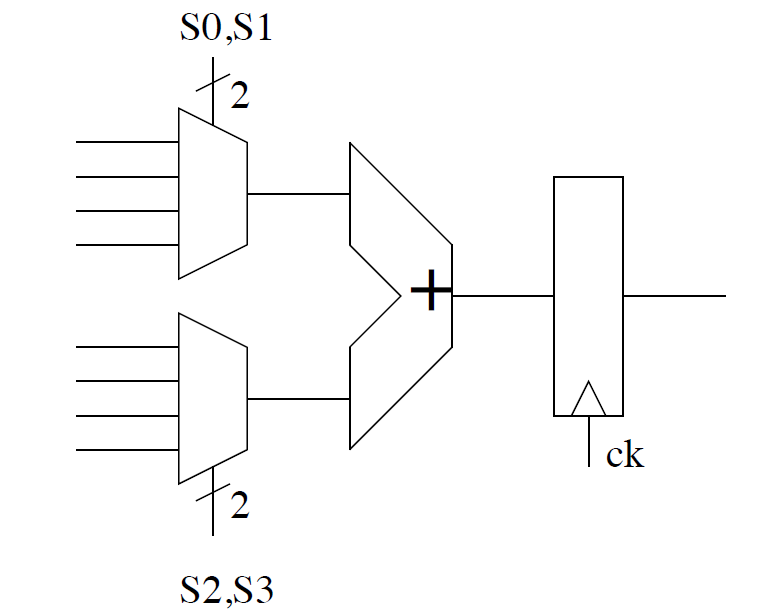
\includegraphics[scale=0.6]{immagini/circuito}
	\caption{\textit{Probabilità e Switching Activity stimati manualmente}}
	\label{datapath}
\end{figure} \\
Dopo varie ottimizzazioni, si è arrivati ad avere un'attività totale pari a 8 per il multiplexer e 6 per la State transition della macchina a stati, andando a considerare che la macchina a stati e il multiplexer ricomincino le operazioni una volta terminate. Nella tabella \ref{tab2} viene riportata la configurazione degli stati e dei bit del multiplexer scelta:
\begin{table}[!h]\footnotesize
	\centering
	\begin{tabular}{|c|c|}
		\hline
		\textbf{STATI} & \textbf{$S_{3}S_{2}S_{1}S_{0}$}\\
		\hline
		000 & 0000\\
		\hline
		001 &0101 \\
		\hline
		011& 0111\\
		\hline
		010& 1110\\
		\hline
		110& 1010\\
		\hline 
	\end{tabular}
	\caption{\textit{Risultati simulazione}}
	\label{tab2}
\end{table} \\
\section{VHDL synthesis}
Il secondo punto del laboratorio prevede di sintetizzare l’FSM tramite synopsys e studiarne le caratteristiche in termini di area, potenza e timing in modo da ricercare possibili ottimizzazioni.\\
Si è utilizzata la libreria a $45 nm$, definito un segnale di clock di periodo corrispondente a $10 ns$, si è verificato il corretto inserimento tramite il comando \emph{report_clock} e si è sintetizzato il circuito.\\
